% !TEX root = ../main.tex

\chapter{Segmentation and preprocessing scripts}
\label{ch:preprocscripts}
This chapter presents the two core contributions of this work. First, a small introduction about the conversion of images is shown. The first main contribution is then explained. It consists of a new module that creates automatically the segmentation masks given the contour of a tumor. The second contribution is the preprocessing of the data itself. For each of the three datasets presented in the Chapter~\ref{ch:datasets}, the preprocessing is explained in detail. All code is written in the Python programming language and publicly available on GitHub\footnote{\url{https://github.com/ChristopheBroillet/Hydra_Segmentation}}.

\section{Images conversion}
\label{sec:imgconversion}
In computer science, images are stored as tables of numbers. Each cell in the table corresponds to one pixel in the image, and contains a certain value (number) that represents the pixel intensity, i.e. the strength of the pixel in a the given type of image. An image can have one or more channels, i.e. layer of pixels, that are stacked to form the image. Three of the most used types of image are:
\begin{enumerate}
  \item The \emph{monochrome image}, also called binary image, contains a binary intensity that is either on or off, and can be interpreted as black and white image. The pixels have either the value 0 (black) or the value 1 (white). The monochrome image is thus encoded in 1 bit per pixel, and has only one channel.
  \item The \emph{greyscale image} contains only intensities on a grey scale. The difference with the monochrome image is that the grey color has many shades and not only 2. The pixel intensity represents then the level of grey of the pixel, and the value depends on the encoding. For example, if a greyscale image is encoded in 8 bits per pixel, the range of the pixel intensity will be $[0,255]$. Here, the black pixel corresponds to the value 0 and the white to the 255 value. The greyscale image has also only one channel.
  \item The \emph{red green blue (RGB) image} is a color image. To represents the colors, shades of red, green and blue are added. The pixel intensity depends on the encoding too. The RGB image contains 3 channels, one for the red, one for the green and one for the blue. These 3 channels are then stacked to form the RGB image. In that case, a pixel is not represented by only one value, as in the two previous types, but by a tuple of three values, one for each RGB colors.
\end{enumerate}

As stated in Section~\ref{sec:dicom}, the DICOM standard aims to standardize all medical images and data between medical institutions worldwide. DICOM converts images with information contained in DICOM tags. The conversion described below is applied on the \texttt{pixel data (7fe0,0010)} DICOM tag, that contains one or more medical images, and will result in converted output images. The conversion is done in two steps that are explained below, while the corresponding code of this work is written in the \texttt{normalize\_dicom} module available on GitHub\footnote{\url{https://github.com/ChristopheBroillet/Hydra_Segmentation/blob/main/preprocessing_scripts/Head-Neck-PET-CT/normalize_dicom.py}}.

\subsection{Hounsfield correction}
The \emph{Hounsfield units} (HU) are universally used units in CT or PET scans, to display a standardized image. The Hounsfield scale is based on the measure of the radiodensity, i.e. the ability of electromagnetic waves to go through a given material. The arbitrarily defined radiodensity of the distilled water (at standard temperature and pressure) is 0~HU, while radiodensity of air is -1000~HU~\cite{schneider_calibration_1996}.

To convert a CT or PET scan, the raw data pixels are first converted using the Hounsfield correction. The equation used to convert original data to HU is given by:
\begin{equation}
  HU = m \cdot P + b
\end{equation}
where $HU$ is the output value in Hounsfield unit, $m$ is the rescale slope given in the \texttt{rescale slope (0028,1053)} DICOM tag, $P$ the input value of the pixel and $b$ the rescale intercept given in the \texttt{rescale intercept (0028,1052)} DICOM tag.

The use of the Hounsfiels units have helped radiologists to interpret and diagnose disease on CT or PET scans. Indeed, scanners take images that have in principle between 12 and 16 bits per pixel, that is between 4096 to 65536 shades of grey. But human eyes struggle to distinguish this amount of shades, while medical displays support encodings from 8 to 10 bits per pixel nowadays. To avoid these two problems, CT and PET scans are converted using the Hounsfield units~\cite{kimpe_increasing_2007}.

\subsection{Normalization}
After this first correction in HU, another linear transformation needs to be applied. This second transformation is necessary in order to keep a normalized output range value $[y_{min},y_{max}]$ for the pixels. To get this output range, the following rules\footnote{These rules are taken from the DICOM standard browser: \\ \url{https://dicom.innolitics.com/ciods/ct-image/voi-lut/00281050}} will be applied to the resulting $HU$ from the first correction for CT and PET scans. For other modalities, they will be applied directly on the pixel values of the image:
\begin{align}
  \begin{split}
    \text{if } HU &\leq c - 0.5 - \dfrac{w - 1}{2} \text{, then } y = y_{min} \\
    \text{else if } HU &> c - 0.5 + \dfrac{w - 1}{2} \text{, then } y = y_{max} \\
    \text{else } y &= \left( \dfrac{HU - (c - 0.5)}{w - 1} + 0.5 \right) \cdot (y_{max} - y_{min}) + y_{min}
  \end{split}
\end{align}
with $HU$ the input pixel value, $c$ the window center given in the \texttt{window center (0028,1050)} and $w$ the window width in the \texttt{window width (0028,1051)}, $y_{min}$ and $y_{max}$ the minimum and maximum value of the output range, and $y$ the output value.

In this work, the output range value will be $[0,255]$, as the output image will be a greyscale image with 8 bits per pixel. In this case, $y_{min} = 0$ and $y_{max} = 255$.


\section{The \texttt{segmentation\_mask} module}
\label{sec:segmaskmodule}
In this work, a new module is provided: the \texttt{segmentation\_mask} module. The goal of this module is to create a segmentation mask for a medical image, given the contour points of the segmentation of the tumor. These contour points are given as ground truth with the dataset they belong to. With these segmentation masks, the deep learning model can be fed with both medical images and segmentation masks. As explained in the Section~\ref{sec:deeplearning}, the medical images are the inputs of the network and the segmentation masks are the labels. The \texttt{segmentation\_mask} module contains two new functions described in the following paragraphs.

\subsection{The \texttt{mm\_to\_imagecoordinates} function}
\label{sec:mmtocoord}
In some cases, like in the Head-Neck-PET-CT dataset, the segmentation points are given in the Patient-Based Coordinate System (PBCS), that are in absolute distance given in millimeters within the patient body. The PBCS is a 3D orthonormal right-handed system, i.e. where the cross product of a unit vector along a $x$ axis and $y$ unit vector gives a $z$ unit vector. Figure~\ref{fig:pbcs} shows one of the most used PBCS orientation.

\begin{figure}[t!]
  \centering
  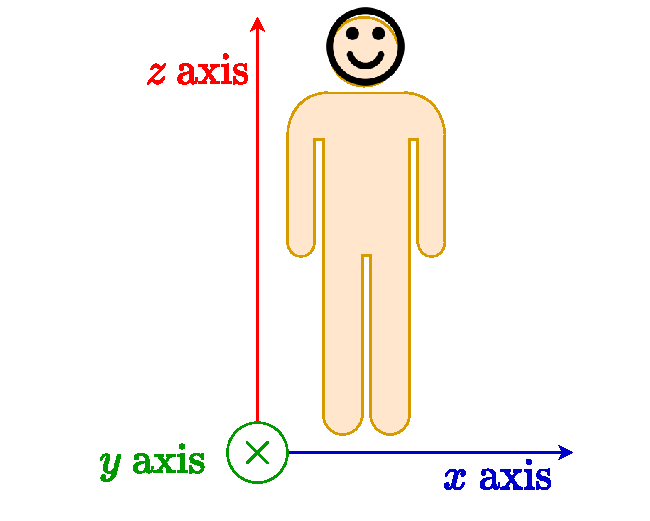
\includegraphics[height=0.25\textheight]{preprocscripts/pbcs.pdf}
  \caption[Patient-base coordinate system orientation example]{Example of an orientation of the patient-base coordinate system. The $x$ axis points from the right to the left of the patient, the $y$ axis from the face to the back of the patient (the axis enters the plane) and the $z$ axis points from the feet to the head of the patient.}
  \label{fig:pbcs}
\end{figure}

The preprocessing and conversion of the images need the row and column indices of the image. The first function of the module, called \texttt{mm\_to\_imagecoordinates}, is used to convert units from the PBCS given in mm, to the image plane coordinate system (IPCS) given in indices. The formula that will be used to convert from one system to the other is taken from the DICOM standard browser\footnote{\url{https://dicom.innolitics.com/ciods/ct-image/image-plane/00200032}}:
% \newpage
\begin{equation}
\label{eq:mmToIndicesMatrix}
  \begin{bmatrix}
    P_x \\ P_y \\ P_z \\ 1
  \end{bmatrix} =
  \begin{bmatrix}
    X_x \Delta_i & Y_x \Delta_j & 0 & S_x \\
    X_y \Delta_i & Y_y \Delta_j & 0 & S_y \\
    X_z \Delta_i & Y_z \Delta_j & 0 & S_z \\
    0 & 0 & 0 & 1 \\
  \end{bmatrix}
  \begin{bmatrix}
    i \\ j \\ 0 \\ 1
  \end{bmatrix}
\end{equation}

The point $(P_x, P_y, P_z)$ represents the coordinates of the point along the three $x,y,z$ axis in the PBCS. It is the point that will be converted in the IPCS. The point given by $(S_x, S_y, S_z)$ is the upper-left pixel in the PBCS, that will be the origin $(0,0,0)$ of the converted image in the IPCS. It is contained in the \texttt{image position (patient) (0020,0032)} DICOM tag. Then, the DICOM tag \texttt{image orientation (patient) (0020,0037)} gives the $(X_x, X_y, X_z, Y_x, Y_y, Y_z)$ values. The $(X_x, X_y, X_z)$ are the direction cosines (i.e. cosines of angles) between the $x$ axis of the Figure~\ref{fig:pbcs} and the row direction of the IPCS. It expresses the change of direction in the PBCS when moving from one column to the next in the IPCS. Similarly, the $(Y_x, Y_y, Y_z)$ are the direction cosines between the $y$ axis of the Figure~\ref{fig:pbcs} and the column direction of the IPCS, and it expresses the change of direction in the PBCS when moving from one row to the next in the IPCS. For example, if the orientation of the PBCS is exactly the one presented in the Figure~\ref{fig:pbcs}, then $(X_x, X_y, X_z, Y_x, Y_y, Y_z)$ will be equal to $(1,0,0,0,1,0)$. Further, the \texttt{pixel spacing (0028,0030)} DICOM tag gives the column spacing $\Delta_i$ between the center of two adjacent pixels in mm, and $\Delta_j$ the row spacing. Finally, $i$ is the \emph{column} index and $j$ the \emph{row} index of the converted image.

As images are in two dimensions, the first two equations of~\eqref{eq:mmToIndicesMatrix} are:
\begin{equation}
  \label{eq:mmToIndicesAlgebra}
  \begin{cases}
    P_x = X_x \Delta_i i + Y_x \Delta_j j + S_x \\
    P_y = X_y \Delta_i i + Y_y \Delta_j j + S_y
  \end{cases}
\end{equation}

The \texttt{solve} method of the \texttt{linalg} module provided by \texttt{NumPy}~\cite{harris_array_2020} is used to solve this system of two equations for $i$ and $j$. The next described function uses the presented function in an optional manner. If the contour points are given in the PBCS, the script needs to call this method to convert the points. If the contour points are already given in the IPCS, then no conversion is required.


\subsection{The \texttt{create\_segmentation\_mask} function}
The second and main function of this module is the \texttt{create\_segmentation\_mask} function. Indeed, this is the function that is primarily called in the preprocessing scripts to start the creation of the segmentation masks. To open and use DICOM files in Python, this function uses the \texttt{pydicom} library~\cite{mason_su-e-t-33_2011}. The outputed segmentation masks are monochrome images. Indeed, black pixels (value 0) represent no tumor, while white pixels (value 1) represent tumor. As arguments, the function takes:
\begin{itemize}
  \item The data contour points of the segmentation. The data needs to be a 2D list, i.e. a list of points $(x,y)$ of the segmentation. The data is considered as ground truth.
  \item The medical image slice that corresponds to the segmentation. This is an opened DICOM file from the \texttt{pydicom} library.
  \item The path to an output folder. This folder will contain the outputed segmentation masks.
  \item A boolean called \texttt{conversion} that indicates if the conversion is required or not. If \texttt{conversion} is \emph{True}, the \texttt{create\_segmentation\_mask} function will use the previous described function in Section~\ref{sec:mmtocoord}.
\end{itemize}
Algorithm~\ref{algo:createsegmask} shows in pseudocode the different steps to create the segmentation masks, by calling the \texttt{create\_segmentation\_mask} function. The following paragraphs explain those steps in detail.

\begin{algorithm}[t!]
  \caption{\texttt{create\_segmentation\_mask} function}
  \label{algo:createsegmask}
  \begin{algorithmic}[1]
    \Function{create\_segmentation\_mask}{$img, data, output\_folder, conversion$}
    \State Create a $log\_file$ \Comment \texttt{.txt} file
    \State Initialize $seg\_mask \gets img \cdot 0$ \Comment 0 for black pixels
    \For{each $point$ in $data$}
      \If{$conversion$} \Comment $conversion$ is a boolean
        \State $x, y \gets$ \texttt{mm\_to\_imagecoordinates}$(img, point)$
      \Else
        \State $x, y \gets point$
      \EndIf
      \State $seg\_mask[y][x] \gets 1$ \Comment Add white pixel
    \EndFor
    \State Initialize $white\_boundaries$\Comment Will contain white indices for each row
    \For{each $white\_row$ in $seg\_mask$}
      \State $white\_boundaries$ append $[row\_idx, min\_white\_idx, max\_white\_idx]$
    \EndFor
    \State Sort $white\_boundaries$ by $row\_idx$
    \State \Comment Two rows at a time, row counter incremented by 1 at each iteration
    \For{each $first, second$ in $white\_boundaries$}
      \If{$first$ and $second$ not differ by 1 in their indices} \Comment Missing line
        \State Add missing line with average value of $first$ and $second$
        \State Write entry in $log\_file$
      \EndIf
    \EndFor
    \State \Comment Three rows at a time, row counter incremented by 1 at each iteration
    \For{each $first, second, third$ in $white\_boundaries$}
      \State $average \gets average(first, second)$
      \State Define $ERROR\_THRESHOLD = 0.05$ \Comment Tolerate to 5\% error
      \If{$\left| \frac{average - second}{average} \right| > ERROR\_THRESHOLD$} \Comment Absurd value
        \State $second \gets average$
        \State Write entry in $log\_file$
      \EndIf
    \EndFor
    \State Sort $white\_boundaries$ by $row\_idx$
    \State Fill white rows in $seg\_mask$ according $white\_boundaries$
    \State \Return{$seg\_mask$}
    \EndFunction
  \end{algorithmic}
\end{algorithm}

At first, an empty mask is initialized, with all pixels value to be 0 (black pixels). This mask will have the same size as the medical image. Then, the contours points given as argument of the function are drawn on the mask as white pixels (value 1). At the same time, a simple log file is created to keep track of the modifications and potential errors occuring during the second step.

The data contour points given with datasets can be partially missing or wrong. Indeed, data is entered by humans and can be the source of mistakes. Data transmission between medical institutions, as well as digitization of old data can also lead to errors. During the second step, the data of the contour points is thus imputed and mitigated if necessary. The presented module first proceeds to imputation, i.e. looks at missing data. It checks if there is a missing line among the contour by looking at the row indices of two consecutive lines. If a line is missing, it looks at the neighbour lines and compute their average white boundaries. The white boundaries delimit the section of a row that contains white pixel. Finally, an entry in the log file is added, specifiying which line was missing.

After imputation of the data, i.e. completing the potential missing rows, the function will then start a data mitigation process, to look for absurd values. It will look at three rows at a time for each iteration step, and compute the average value of the first and third line. This computed value will then be compared with the value of the second (middle) line. If the comparison results in a too big difference between the values, defined by a threshold, the middle value is considered as an error or an absurd value. In this work, a too big difference (absurd value) is when values of white boundaries differ from more than 5\% than their neighbours. The data is then mitigated by replacing the old value with the neighbour average value, and an entry is added to the log file, with the old and new values.

Figure~\ref{fig:segmasklog} shows an example log file for an image of the HNPC dataset. The HNPC contained some missing lines and absurd values in the data extracted from the RTStruct series, while the LIDC-IDRI dataset had no errors.

\begin{figure}[t!]
  \centering
  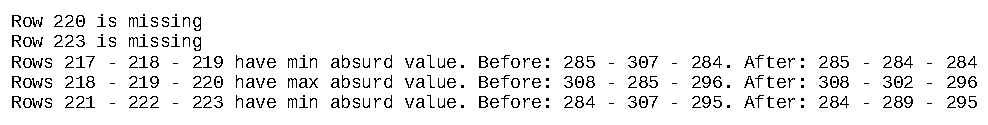
\includegraphics[width=\textwidth]{preprocscripts/segmasklog.pdf}
  \caption[Example log file from the \texttt{create\_segmentation\_mask} function]{Example log file from the \texttt{creste\_segmentation\_mask} function. This file tells the user that the rows 220 and 223 were missing in the original data, and were added by the function. Then, the function mitigated some values that had more than 5\% error. The file shows the old and new values.}
  \label{fig:segmasklog}
\end{figure}

The following sections will present and explain the preprocessing Python scripts for the new datasets, in both textual information or in pseudocode. To manage the DICOM files contained in the datasets but also to get the access to the DICOM tags, the scripts will use the \texttt{pydicom} library.

\section{LIDC-IDRI preprocessing}
\label{sec:lidcpreproc}
In order to use this dataset for a supervised learning training purpose, the images and the medical diagnoses have to be preprocessed first. Because of simplicity and completeness of the data and their labels in the dataset, this work only considers the first category (Nodules >= 3 mm). The other two categories are left out.

The LIDC-IDRI dataset can be used for two different tasks. The first task will be the \emph{localization} task, to detect if the nodules are cancerous or not, and also locate them within the image. The second task will be the \emph{segmentation} task, where the contour of the cancerous nodule will be drawn. The preprocessing is done in a single step, where the images are converted from DICOM to \texttt{NumPy} arrays, and the labels are collected. For each slice, the label for the localization task will be a True/False diagnosis and the location of the center of the nodule, as the label for the segmentation task will be a segmentation mask. For the preprocessing of this dataset, only one script has been written. When running it, the user is first asked to enter the task he wants to perform, either the localization or the segmentation. The script then performs the given task.

\subsubsection{Preprocessing for the localization task}
The idea of the preprocessing for the localization is to first classify in a binary manner the nodules according their malignancy, given in a 1 to 5 scale by the radiologists, 1 being benign and 5 being malignant. The nodules that have a malignancy of 1 or 2 are treated as False cases, while the nodules with a malignancy of 4 or 5 are treated as True cases. The nodules with malignancy 3 are left aside as the diagnosis is uncertain.

Then, for each of this cases, the corresponding slice is searched and taken. As the contour is given in a XML file for each of these slices, the $x$ and $y$ coordinates are extracted, and the center of the nodule is computed, via a mean calculation. The slices are finally converted into greyscale images encoded in 8 bits per pixel (pixel intensity from 0 to 255) using the conversion steps of Section~\ref{sec:imgconversion}. The script does this conversion so that the slice can be displayed correctly on a screen. The center of the nodule is saved in the name of the file, and the True and False cases are separated in two different output folders. For example, a True case can have the name \texttt{LIDC-IDRI-0001\_nid-0\_pos-314-365\_29.npy}. The first part, \texttt{LIDC-IDRI-0001} is the patient ID, \texttt{nid-0} is the nodule ID as the case can have more than one nodule. Then, the position of the center of the nodule \texttt{pos-314-365} is given in $(x,y)$ coordinates. Finally, the last number \texttt{29} is an added index to avoid duplicate names. The different steps to preprocess the dataset for the localization are shown in the Algorithm~\ref{algo:lidcpreproclocalization}.

\begin{algorithm}[t!]
  \caption{LIDC-IDRI preprocessing for the \emph{localization} task}
  \label{algo:lidcpreproclocalization}
  \begin{algorithmic}[1]
    \State Create two folders $True$ and $False$ in $output\_folder$
    \For{each $series$ in $dataset\_folder$} \Comment{Iterate over patients/studies/series}
      \If{$series$ is not CT}
        \State Continue
      \EndIf
      \State Initialize $nodules\_df['Nodule ID', 'x pos', 'y pos', 'z pos', 'Diagnosis']$
      \State Get the 4 $reading\_sessions$ of the radiologists \Comment{By parsing XML file}
      \For{each $session$ in $reading\_sessions$}
        \For{each $nodule$ in $session$}
          \If{malignancy in [1,2]}
            \State $diagnosis = False$
          \ElsIf{malignancy in [4,5]}
            \State $diagnosis = True$
          \Else
            \State Continue
          \EndIf
          \State Initialize $x\_coords = []$ and $y\_coords = []$
          \For{each $slice$ in $nodule$}
            \For{each $contour\_point$ in $slice$}
              \State $[x, y] \gets contour\_point$ \Comment{Get coordinates}
              \State $x\_coords$ append $x$
              \State $y\_coords$ append $y$
            \EndFor
            \State $x\_mean \gets mean(x\_coords)$
            \State $y\_mean \gets mean(y\_coords)$
            \State $z \gets slice$
            \State $nodules\_df$ append $[NoduleID, x\_mean, y\_mean, z, Diagnosis]$
          \EndFor
        \EndFor
      \EndFor
      \For{each $row$ in $nodules\_df$}
        \For{each $dicom\_image$ in $patient$}
          \If{$dicom\_image$ is the slice where the nodule of $row$ appears}
            \State $diagnosis \gets row['Diagnosis']$
            \State $slice \gets normalize(dicom\_image)$ \Comment{\texttt{normalize\_dicom} module}
            \State Save $slice$ in $output\_folder/\{diagnosis\}$
          \EndIf
        \EndFor
      \EndFor
    \EndFor
  \end{algorithmic}
\end{algorithm}

\subsubsection{Preprocessing for the segmentation task}
The preprocessing for the segmentation task is very similar to the preprocessing for the localization task, as it uses the same dataset. The script for the localization task took the nodules of the first category (Nodules >= 3 mm) with malignancy 1, 2, 4 or 5. For the segmentation however, the script only takes the cancerous nodules, i.e. with malignancy 4 or 5. The other ones are left out.

Then, the XML parsing is done in the very same way as the localization task, by getting all contour points, but this time the center of the nodules is not computed, as only the contour points themselves are required to do the segmentation task. These contour points are then saved in a list.

Finally, the images are converted into greyscale images encoded in 8 bits per pixel, and the segmentation masks, that are monochrome images, are created using the \texttt{segmentation\_mask} module. Algorithm~\ref{algo:lidcpreprocsegmentation} shows the steps to preprocess the dataset for the segmentation task.

\begin{algorithm}[t!]
  \caption{LIDC-IDRI preprocessing for the \emph{segmentation} task}
  \label{algo:lidcpreprocsegmentation}
  \begin{algorithmic}[1]
    \State Create two folders $img$ and $masks$ in $output\_folder$
    \For{each $series$ in $dataset\_folder$} \Comment{Iterate over patients/studies/series}
      \If{$series$ is not CT}
        \State Continue
      \EndIf
      \State Initialize $nodules\_df['Nodule ID', 'contour data', 'z pos']$
      \State Get the 4 $reading\_sessions$ of the radiologists \Comment{By parsing XML file}
      \For{each $session$ in $reading\_sessions$}
        \For{each $nodule$ in $session$}
          \State Select nodules of malignancy $\geq 4$
          \State Initialize $contour\_points = []$
          \For{each $slice$ in $nodule$}
            \For{each $contour\_point$ in $slice$}
              \State $[x, y] \gets contour\_point$ \Comment{Get coordinates}
              \State $contour\_points$ append $[x, y]$
            \EndFor
            \State $z \gets slice$
            \State $nodules\_df$ append $[NoduleID, contour\_points, z]$
          \EndFor
        \EndFor
      \EndFor
      \For{each $row$ in $nodules\_df$}
        \For{each $image$ in $patient$}
          \If{$image$ is the slice where the nodule of $row$ appears}
            \State $image\_slice \gets normalize(image)$ \Comment{\texttt{normalize\_dicom} module}
            \State Save $image\_slice$ in $output\_folder/img$
            \State $segmentation\_mask \gets create\_segmentation\_mask$
            \State Save $segmentation\_mask$ in $output\_folder/masks$
          \EndIf
        \EndFor
      \EndFor
    \EndFor
  \end{algorithmic}
\end{algorithm}

\newpage
\section{HNPC preprocessing}
The preprocessing of the Head-Neck-PET-CT dataset is separated in two phases. In the first phase, the preprocessing script iterates over all patients, studies and series. It then checks the modality of the series. If the series is a CT or PET series (image series) or a RTStruct series, the script continues. If the modality is something else, like RTDose or RTPlan, the series is just skipped as the script does not need it to preprocess for the segmentation task.

Then, the script reads the spreadsheet \texttt{INFO\_GTVcontours\_HN.xlsx}, and extracts the names the radiologists gave to the tumors. For both types of image series (CT and PET), the script saves the Patient ID, the series universal identifier (UID), the modality, the path and the roi name of the tumor in a \texttt{pandas}~\cite{the_pandas_development_team_pandas-devpandas_2020, mckinney_data_2010} dataframe. In addition, for the RTStruct series only, the script also saves the series UID of its referenced image series. In that way, the dataframe contains names, UID and relations between the RTStruct series and their corresponding images. This will make it easier to work with in the next step.

In the second phase, the \texttt{pandas} dataframe just created is separated in two other dataframes: one containing only the images series, and the other containing the \mbox{RTStruct} series. An iteration is then started in the RTStruct dataframe. The goal of this iteration is to first take the RTStruct and its corresponding images series, and for each slice of the images series that contains the tumor, it then extracts the contour points that segment the tumor. Finally, the image is as before converted into a \texttt{NumPy} array, and the contour points are inputed into the \texttt{segmentation\_mask} module, which outputs the segmentation mask. The Algorithm~\ref{algo:hnpcpreproc} shows all this preprocessing.

\begin{algorithm}[t!]
  \caption{HNPC preprocessing}
  \label{algo:hnpcpreproc}
  \begin{algorithmic}[1]
    \State Create two folders $img$ and $masks$ in $output\_folder$
    \State Initialize $metadata\_df$
    \State Read excel file $roinames\_excel$ \Comment{\texttt{INFO\_GTVcontours\_HN.xlsx}}
    \For{each $patient$ in $dataset\_folder$}
      \For{each $visit$ in $patient$}
        \For{each $series$ in $visit$}
          \If{$series$ is CT, PET or RTStruct}
            \State $metadata\_df$ append metadata information
          \EndIf
        \EndFor
      \EndFor
    \EndFor
    \State Split $metadata\_df$ in $RT\_df$, $images\_df$ \Comment according to modality
    \For{each $row$ in $RT\_df$}
      \State $dicom\_file \gets row$
      \State Open $dicom\_file$ \Comment{Get $ROI\_contour\_sequence$}
      \For{each $contour\_sequence$ in $ROI\_contour\_sequence$}
        \State $contour\_image \gets contour\_sequence[0\text{x}3006,0\text{x}16][0]$ \Comment{DICOM tag}
        \State $series\_images\_path \gets contour\_image[0\text{x}8,0\text{x}1155].value$ \Comment{DICOM tag}
        \For{each $image$ in $series\_images\_path$}
          \State $dicom\_image \gets$ Search the referenced slice
          \State $image\_slice \gets normalize(dicom\_image)$ \Comment{\texttt{normalize\_dicom} module}
          \State Save $image\_slice$ in $output\_folder/img$
          \State $segmentation\_mask \gets create\_segmentation\_mask$
          \State Save $segmentation\_mask$ in $output\_folder/masks$
        \EndFor
      \EndFor
    \EndFor
  \end{algorithmic}
\end{algorithm}

\newpage
\section{BUSI preprocessing}
The preprocessing steps of BUSI are much shorter than in the two previous datasets. As the images are given in the PNG format, the preprocessing script does no use the \texttt{pydicom} library. While the segmentation masks have already been created and given in the dataset, the script does not use either the \texttt{segmentation\_mask} module. No resizing or rescaling operation is needed, as images and masks are already in the same size. Thus, a simple conversion from PNG to \texttt{NumPy} array is required to preprocess this dataset. As the segmentation masks for the images of the first category (normal) are empty, this category is not taken in the preprocessing.

For both remaining categories (benign and malignant), the preprocessing script iterates over the original images. It can then find the corresponding segmentation masks, as they have the same name as the images. Once the image and its mask are found, they are converted into \texttt{NumPy} arrays, in format of 8 bits per pixel, 1-channel greyscale. They are finally saved under two distinct folders, one for the images and one for the masks. The preprocessing of the BUSI dataset is already finished. The Algorithm~\ref{algo:busipreproc} shows the different steps to preprocess the BUSI dataset.

\begin{algorithm}[t!]
  \caption{BUSI preprocessing}
  \label{algo:busipreproc}
  \begin{algorithmic}[1]
    \State Create two folders $img$ and $masks$ in $output\_folder$
    \For{each $category$ in $dataset\_folder$}
      \If{$category = normal$}
        \State Continue
      \EndIf
      \State $image\_paths\_list \gets$ Get all original images of $category$
      \For{$image\_path$ in $image\_paths\_list$}
        \If{$image\_name$ matches $image\_path$} \Comment With a RegEx
          \State Construct $mask\_name$ and $mask\_path$ from $image\_name$
          \State $image\_slice \gets convert(image\_path)$
          \State Save $image\_slice$ in $output\_folder/img$
          \State $segmentation\_mask \gets convert(mask\_path)$
          \State Save $segmentation\_mask$ in $output\_folder/masks$
        \EndIf
      \EndFor
    \EndFor
  \end{algorithmic}
\end{algorithm}


\section{Discussion}
This work improves the Hydra framework in the following ways:
\begin{itemize}
  \item The new \texttt{segmentation\_mask} module provides a robust way to create segmentation masks, given a medical image and the contour points of the tumor. The module is ready to be used for other future datasets for the segmentation task, and will give the segmentation masks for each image. Even if the contour points data is not complete or have some absurd values, the module will impute and mitigate the missing data. The \texttt{segmentation\_mask} outputs two different files. On one hand, the segmentation masks that are monochrome images, will represent the labels during the training of Hydra, in a supervised learning manner. On the other, each mask will have a proper log file containing information about the imputation and mitigation of the data if necessary. The user can check these log files for a debugging purpose, and to see where data contained errors. Finally, the proper segmentation mask is created and returned along with the preprocessed medical image.
  \item The \texttt{segmentation\_mask} module can also be used to segment other objects than just tumors. For example, if a CAD system is designed to segment the prostate itself as in the \emph{PROMISE12} challenge (see Section~\ref{sec:cadsegtask}), then this module is ready to output a mask that segments the prostate, and can be easily added to this CAD system.
  \item Hydra can now uses new datasets. Indeed, after all the preprocessing steps presented in this work that are implemented in three different preprocessing scripts, the three datasets are now ready to be used to train the Hydra model. Firstly, the \emph{lung image database collection} can be used either for the localization task, or the segmentation task. A single script preprocesses this dataset for the two tasks. Then, the \emph{head-neck-PET-CT} and the \emph{breast ultrasound images} datasets can both be used for the segmentation task. At the end, each medical image has its own corresponding segmentation mask as ground truth, and they can be used together to train the segmentation task in a supervised learning manner.
  \item The \texttt{normalize\_dicom} has received some minor changes. The code has been cleaned to be more readable by the user, but it basically achieves the same goal: convert the medical images in a standardized manner, with or without the use of the Hounsfield units, and in a way that Hydra can read.
\end{itemize}
